\textbf{Цель:} Измерение скорости звука в воздузе методом стоячей волны.

\textbf{Принадлежности:} установка, звуковой генератор.

\begin{center}
    \textbf{Описание установки и вывод рабочей формулы.}
\end{center}

Для определения скорости звука методом стоячей волны используют установку показанную на (рис \ref{fig:установка_13_2})

\begin{figure}[!h]
    \centering
    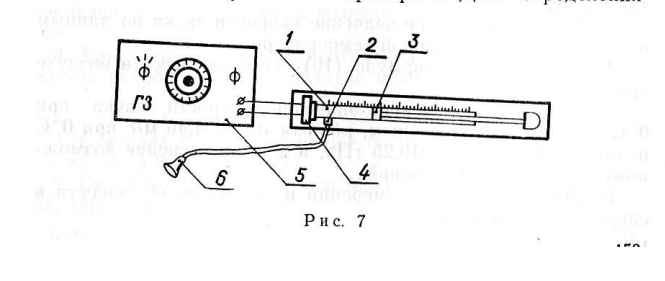
\includegraphics[width = 0.5\textwidth]{image/image13_2.png}
    \caption{Установка для Определения отношения молярных теплоемкостей газа адиабатическим методом.}
    \label{fig:установка_13_2}
\end{figure}

Длина волны вычисляется по следующей формуле(\ref{eq:formula_13_2_1}):

\begin{equation}
    \lambda = 2 \frac{l_2 - l_1}{n}
    \label{eq:formula_13_2_1}
\end{equation}

где $l_1$ "--- положение поршня по шкале, соответствующее первому максимуму громкости звука, $l_2$ "--- соответствующее $n+1$ максимуму, $n$ "--- число полуволн на расстоянии $l2-l1$.

В этом случае на расстоянии $l_2 - l_1$ должно укладываться $n$ полуволн  $\lambda / 2$.

Тогда величина скорости звука запишется выражением(\ref{eq:formula_13_2_2}):

\begin{equation}
    \upsilon = \lambda \nu = 2 \frac{l_2 - l_1}{n} \nu
    \label{eq:formula_13_2_2}
\end{equation}

где $\nu$ "--- частота колебаний генератора.

\begin{center}
    \textbf{Порядок выполнения работы.}
\end{center}

\begin{enumerate}
    \item{Включить в сеть звуковой генератор.}
    \item{Установить одну из трех заданных преподавателем частот от 1400 до 2000 Гц.}
    \item{Перемещая поршень 3 за отросток 2, заметить по шкале положение поршня l1, соответствующее первому максимуму громкости звука, фиксируемое с помощью слуховой трубки 6.}
    \item{Перемещая поршень к правому краю трубки 1, заметить положение поршня $l_2$, соответствующее $n+1$ максимуму звука.}
    \item{Измерения $l_1$ и $l_2$ проделать не менее трех раз (\ref{tab:1400_гц_table}).

            \begin{table}[h!]
                \centering
                \begin{tabular}{|c|c|c|c|}
                    \hline
                    $l_1$ & $0.253$ м & $0.498$ м & $0.742$ м \\
                    \hline
                    $l_2$ & $0.376$ м & $0.621$ м & $0.865$ м \\
                    \hline
                \end{tabular}
                \caption{измерения при 1400 Гц}
                \label{tab:1400_гц_table}
            \end{table}
        }
    \item{Провести измерения, указанные в пунктах 2--5 для двух других частот(\ref{tab:1700_гц_table}), (\ref{tab:2000_гц_table}).

            \begin{table}[h!]
                \centering
                \begin{tabular}{|c|c|c|c|}
                    \hline
                    $l_1$ & $0.207$ м & $0.41$ м & $0.612$ м \\
                    \hline
                    $l_2$ & $0.31$ м & $0.511$ м & $0.713$ м \\
                    \hline
                \end{tabular}
                \caption{измерения при 1700 Гц}
                \label{tab:1700_гц_table}
            \end{table}

            \begin{table}[h!]
                \centering
                \begin{tabular}{|c|c|c|c|}
                    \hline
                    $l_1$ & $0.263$ м & $0.435$ м & $0.606$ м \\
                    \hline
                    $l_2$ & $0.349$ м & $0.522$ м & $0.693$ м \\
                    \hline
                \end{tabular}
                \caption{измерения при 2000 Гц}
                \label{tab:2000_гц_table}
            \end{table}
        }
    \item{Вычислить значения скорости звука по рабочей формуле(\ref{eq:formula_13_2_2})

            1400 Гц:

            $\upsilon_1 = 2 \frac{0.376 - 0.253}{1} 1400 = 344.4 \frac{\text{м}}{\text{с}}$;

            $\upsilon_2 = 2 \frac{0.621 - 0.498}{1} 1400 = 344.4 \frac{\text{м}}{\text{с}}$;

            $\upsilon_1 = 2 \frac{0.865 - 0.742}{1} 1400 = 344.4 \frac{\text{м}}{\text{с}}$;

            1700 Гц:

            $\upsilon_1 = 2 \frac{0.31 - 0.207}{1} 1700 = 350.2 \frac{\text{м}}{\text{с}}$;

            $\upsilon_2 = 2 \frac{0.511 - 0.41}{1} 1700 = 343.4 \frac{\text{м}}{\text{с}}$;

            $\upsilon_3 = 2 \frac{0.713 - 0.612}{1} 1700 = 343.4 \frac{\text{м}}{\text{с}}$;

            2000 Гц:

            $\upsilon_1 = 2 \frac{0.349 - 0.263}{1} 2000 = 344 \frac{\text{м}}{\text{с}}$;

            $\upsilon_2 = 2 \frac{0.522 - 0.435}{1} 2000 = 348 \frac{\text{м}}{\text{с}}$;

            $\upsilon_1 = 2 \frac{0.693 - 0.606}{1} 2000 = 348 \frac{\text{м}}{\text{с}}$;
        }
    \item{Вычислить средние значения скорости звука по данным всех измерений при данной температуре.

            $\upsilon_\text{1400ср} = \frac{344.4 + 344.4 + 344.4}{3} = 344.4 \frac{\text{м}}{\text{с}}$;

            $\upsilon_\text{1700ср} = \frac{350.2 + 343.4 + 343.4}{3} = 345.(6) \frac{\text{м}}{\text{с}}$;

            $\upsilon_\text{2000ср} = \frac{344 + 348 + 348}{3} = 346.(6) \frac{\text{м}}{\text{с}}$;
        }
    \item{Рассчитать  по формуле (\ref{eq:formula_13_2_3}) скорость  звука в воздухе при $0^o$С.

            \begin{equation}
                \upsilon_0 = \frac{\upsilon}{\sqrt[2]{1 + \alpha t}}
                \label{eq:formula_13_2_3}
            \end{equation}

            $\upsilon_{0.1} = \upsilon_{0.2} = \upsilon_{0.3} = \frac{344.4}{\sqrt[2]{1 + 0.004 \cdot 21}} = 330.787 \frac{\text{м}}{\text{с}}$;

            $\upsilon_{0.4} = \frac{350.2}{\sqrt[2]{1 + 0.004 \cdot 21}} = 336.357 \frac{\text{м}}{\text{с}}$;

            $\upsilon_{0.5} = \upsilon_{0.6} = \frac{343.4}{\sqrt[2]{1 + 0.004 \cdot 21}} = 329.826 \frac{\text{м}}{\text{с}}$;

            $\upsilon_{0.7} = \frac{344}{\sqrt[2]{1 + 0.004 \cdot 21}} = 330.402 \frac{\text{м}}{\text{с}}$;

            $\upsilon_{0.8} = \upsilon_{0.9} = \frac{348}{\sqrt[2]{1 + 0.004 \cdot 21}} = 334.244 \frac{\text{м}}{\text{с}}$;

            \textbf{Средние значения:}

            \textbf{1400 Гц:} $330.787 \frac{\text{м}}{\text{с}}$;

            \textbf{1700 Гц:} $332.003 \frac{\text{м}}{\text{с}}$;

            \textbf{2000 Гц:} $332.96(3) \frac{\text{м}}{\text{с}}$;
        }
    \item{Сравнить полученное значение скорости звука при $0^o$С с табличным значением, равным $\upsilon_0 = 331.46 \frac{\text{м}}{\text{с}}$; при $0_o$С и давлении воздуха $1013.25$ гПа, и дать объяснение возможному расхождению значений.

            \begin{center}
                $\upsilon = \lambda \nu = 2 \frac{l_2 - l_1}{n} \nu =>$

                $\ln \left (\upsilon \right ) = \ln \left (2 \frac{l_2 - l_1}{n} \nu \right ) = \ln \left (2 \right ) + \ln \left (l_2 - l_1 \right ) - \ln \left (n \right ) + \ln \left (\nu \right ) =>$

                $\frac{\Delta \upsilon}{\upsilon} = 0 + \frac{\Delta \left(l_2 - l_1 \right )}{l_2 - l_1} - \frac{\Delta n}{n} + \frac{\Delta \nu}{\nu} =>$

                $\frac{\Delta \upsilon}{\upsilon} = \frac{l_1 \Delta l_2 - l_2 \Delta l_1}{l_2 - l_1} - \frac{\Delta n}{n} + \frac{\Delta \nu}{\nu}$,
            \end{center}
            где $\Delta l_1 = \Delta l_2 = 0.001 \text{м}$, $\Delta \nu = 1$, $\Delta n = 1$.

            Тогда формула принимает вид:

            $\frac{\Delta \upsilon}{\upsilon} = \frac{0.001 l_1 - 0.001 l_2}{l_2 - l_1} - \frac{1}{n} + \frac{1}{\nu}$,

            n "--- количество полу волн, $\nu$ "--- частота

            Но т. к. n в нашем случае всегда равен 1, и в силу простых преобразований можем изменить формулу:

            $\frac{\Delta \upsilon}{\upsilon} = \frac{0.001 \left(l_1 - l_2 \right )}{l_2 - l_1} - 1 + \frac{1}{\nu} = \frac{-0.001 \left (l_2 - l_1 \right )}{l_2 - l_1} - 1 + \frac{1}{\nu}$

            (пояснение то что идет дальше: т. к. $n = 1$ всегда, то $n = const$, поэтому мы это просто убираем и не паримся, получая норм погрешность (\textbf{ЭТО НАДО УДАЛИТЬ И КАК-ТО СВОИМИ СЛОВАМИ НАПИСАТЬ}))

            Тогда для частот 1400, 1700 и 2000 Гц имеют место вычисления:

            1400:

            $|-0.001 + \frac{1}{1400}| = \frac{3501}{3500} \approx 0.000285714$;

            1700:

            $|-0.001 + \frac{1}{1700}| = \frac{17007}{17000} \approx 0.00041$;

            2000:

            $|-0.001 + \frac{1}{2000}| = \frac{2001}{2000} \approx 0.0005$.

            Это и есть $\delta_\text{м}$ для данных частот.

            Найдем $\delta_\text{э}$ согласно формуле

            $\delta_\text{э} = \frac{\upsilon^\text{теор}_0 - \upsilon^\text{экс}_0}{\upsilon^\text{теор}_0} \cdot 100\%$

            Для $\upsilon_0$ у разных частот мы имеем:

            1400:

            $\delta_\text{э} = |\frac{331.46 - 330.787}{331.46}| \cdot 100\% = \frac{673}{331460} \cdot 100\% \approx 0.203041\%$

            1700:

            $\delta_\text{э} = |\frac{331.46 - 332.003}{331.46}| \cdot 100\% = \frac{543}{331460} \cdot 100\% \approx 0.163821\%$

            2000:

            $\delta_\text{э} = |\frac{331.46 - 332.963}{331.46}| \cdot 100\% = \frac{1503}{331460} \cdot 100\% \approx 0.453448\%$

            Для нахождения $\Delta \delta$ воспользуемся формулой $\Delta \delta = \delta_\text{э} - \delta_\text{м}$:

            1400:

            $0.203041 - 0.000285714 = 0.202755286$

            1700:

            $0.163821 - 0.00041 = 0.163411$

            2000:

            $0.453448 - 0.0005 = 0.452948$
        }
    \item{Данные прямых измерений и вычислений занести в следующую таблицу:}
\end{enumerate}





















